\documentclass[a4paper,12pt]{article}
\usepackage[utf8]{inputenc}
\usepackage[english,russian]{babel}
\usepackage{indentfirst}
\usepackage{amsmath}
\usepackage{amssymb}
\usepackage{amsfonts}
\usepackage{amsthm}
\usepackage{graphicx}
\usepackage{subcaption}
\usepackage{systeme,mathtools}
\title{Лабораторная работа №3\\Плавающие объекты: рисунки и таблицы}
\author{БГУ,ММФ,1 курс, 5 группа, Бельская Екатерина Артуровна}
\begin{document}
\maketitle
\section*{Задание 1. Создание таблицы в \LaTeX-документе}

\begin{table}[h!]
\caption{Функция $y=\arccos \frac{2x}{1+x^2}$}
\centering

\begin{tabular}{|c|c|c|}

\hline
Описание функции & $X$ & $Y$\\
\hline \hline
$y=\arccos \frac{2x}{1+x^2}$ & $\mathbb{R}$ & $
\lbrace y\in \mathbb{R} : 0\leqslant y\leqslant \pi\rbrace .$ \\
\hline

\end{tabular}
\label{table:tabl}
\end{table}
Функция $y=\arccos x$ --- это функция, обратная к $x=\cos y$. Она имеет область определения $-1\leqslant x\leqslant 1$ и множество значений $0\leqslant y\leqslant \pi$. В нашем случае в качестве аргумента $x$ выступает выражение $\frac{2x}{1+x^2}$. Оценим данное выражение:
\begin{equation}
	-1\leqslant \frac{2x}{1+x^2}\leqslant 1.
\end{equation} 
Так знаменатель средний дроби ни при каких значениях $x$ не обращается в 0, умножим каждую часть неравенства на ${1+x^2}$ и перейдём к системе неравенств:
\[\left \lbrace
\begin{array}{ll}
-1-x^2-2x\leqslant 0\\
-1-x^2+2x\leqslant0.
\end{array}\right.\]
В результате их решения получаем $\forall x\in\mathbb{R}$ функция $y=\arccos \frac{2x}{1+x^2}$ определена.
\\Так как к функции $y=\arccos \frac{2x}{1+x^2}$ не применяются никакие преобразования, область допустимых значений совпадает с естественной областью допустимых значений функции $\arccos x$.
\newpage
\section*{Задание 2. Импортирование графики в \LaTeX-документ}

\begin{figure}[h]
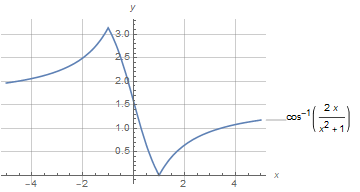
\includegraphics[width=\textwidth]{rastrr.png}
\caption{Растровое изображение функции $y=\arccos \frac{2x}{1+x^2}$}
\label{fig:pic1}
\end{figure}

\begin{figure}[h]
  \centering
  \begin{subfigure}[b]{0.45\linewidth}
    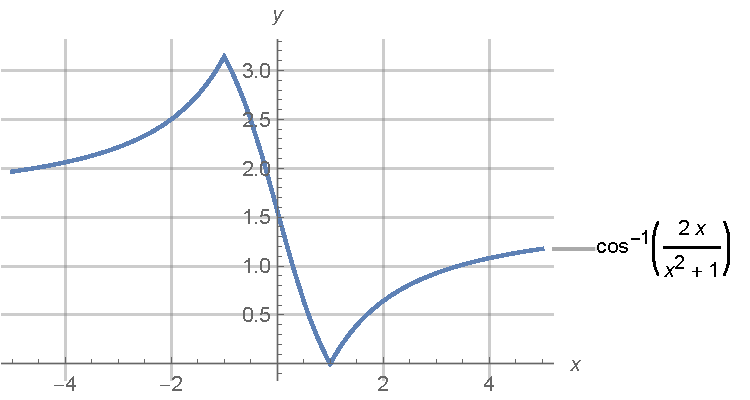
\includegraphics[width=\textwidth,height=5cm]{vect.pdf}
  \end{subfigure}
  \begin{subfigure}[b]{0.45\linewidth}
    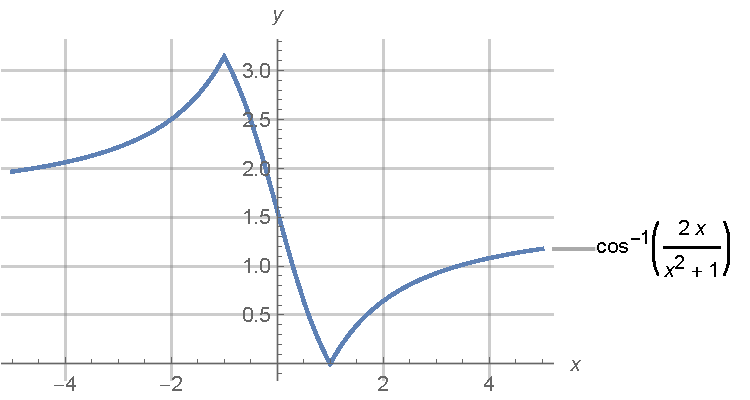
\includegraphics[width=\textwidth,trim={ 0  1cm 5cm 0},clip]{vect.pdf}
  \end{subfigure}
  \caption{Векторное изображение функции $y=\arccos \frac{2x}{1+x^2}$}
   \label{fig:pic2}
\end{figure}

Рис.\ref{fig:pic1} и Рис.\ref{fig:pic2} являются изображениями функции из Таблицы \ref{table:tabl}.

\begin{thebibliography}{7}
\bibitem{Otiker} Отикер~Т. Не очень краткое введение в LaTeX 2е (перевод Б. Тоботрас) --- 2003.
\bibitem{Kotelnikov} Котельников И. А., Чеботаев П. З. LaTeX по-русски (3-е изд.) ---Новосибирск: Сибирский хронограф, 2004.

\end{thebibliography}

\end{document}